\subsection{Score calibration and hidden-set output}
The mixture is an uncalibrated prediction of violation used for ranking. A high predicted score does not exclude a physically good composition. The following in-training diagnostic uses the frozen 02+03 refit on public rows; it is not a generalization estimate.
\begin{table}[htbp]\centering\small\caption{In-training residual diagnostics for the three-family score table. Bias is mean predicted minus observed violation.}\begin{tabular}{lrrrr}\toprule Group & $n$ & Min. prediction & Median prediction & Bias\\\midrule
All public Q3 families & 6525 & 3.268 & 21.371 & -0.048\\
Public NO2 near-targets & 14 & 7.862 & 9.994 & 9.731\\
Public near-targets & 61 & 3.268 & 10.982 & 10.399\\
\bottomrule\end{tabular}\end{table}
The minimum of all 3,703 Q1 hidden scores is 5.099. The organizers report 19 hidden zero-violation targets, so score magnitude must not be interpreted as a calibrated physical measurement.
\begin{figure}[htbp]\centering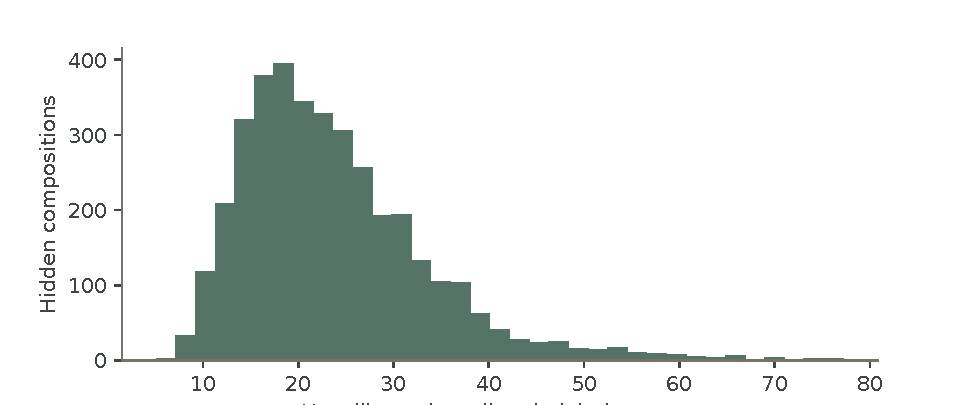
\includegraphics[width=.85\linewidth]{figures/q1_distribution.pdf}\caption{Distribution of Q1 predictions from the 02-only model. Hidden physical labels are unavailable.}\end{figure}
\begin{table}[htbp]\centering\small\caption{First 20 hidden compositions ranked by the Q1 model. All entries are predictions.}\begin{tabular}{rrlr}\toprule Rank & ID & Formula & Score\\\midrule
1 & 5619 & SnZrO2S & 5.0994\\
2 & 18337 & CaNbO2S & 6.6618\\
3 & 5590 & CaTaO2S & 7.2127\\
4 & 2460 & SrNbO2S & 7.2822\\
5 & 3094 & SrNbOFN & 7.3303\\
6 & 18896 & CaNbOFN & 7.4778\\
7 & 11576 & SrTaO2S & 7.4803\\
8 & 6191 & YTiO2S & 7.6029\\
9 & 17664 & BaTaO2S & 7.6791\\
10 & 10869 & CaSnO2S & 7.8212\\
11 & 747 & CaGaO2F & 7.9208\\
12 & 13762 & CdHfO2S & 7.9241\\
13 & 10039 & SrNbO3 & 8.1826\\
14 & 8723 & YTaO2S & 8.2117\\
15 & 12896 & InHfO2S & 8.4206\\
16 & 12933 & BaGaO2F & 8.5014\\
17 & 502 & CaGaO2S & 8.5349\\
18 & 2872 & CaNbO3 & 8.5719\\
19 & 15279 & CaGeO2S & 8.5918\\
20 & 11752 & CaSnO2F & 8.6145\\
\bottomrule\end{tabular}\end{table}
